%% chapitre 1
\documentclass[a4paper,dvips]{article}
\usepackage{ucs}
\usepackage[utf8x]{inputenc}
\usepackage[T1]{fontenc}
\usepackage[dvips]{graphicx}
\usepackage{amsmath}
\usepackage{psfrag}
\usepackage{subfig}
\begin{document}
\begin{figure}[ht]
    \begin{center}
        \psfrag{D}{$D$}
        \psfrag{dD}{$\partial D$}
        \psfrag{M}{$M$}
        \psfrag{n}{$\vec{n}$}
        \psfrag{T}{$\vec{T}$}
        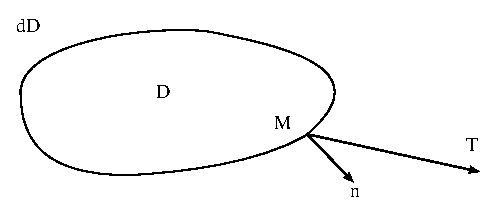
\includegraphics{../images/T1_Ch01-0001}
    \end{center}
    \caption{Efforts de contact}
    \label{fig:T1_Ch01-0001}
\end{figure}
\begin{figure}[ht]
    \begin{center}
        \psfrag{D1}{$D_I$}
        \psfrag{D2}{$D_{II}$}
        \psfrag{D3}{$D_{III}$}
        \psfrag{Vdt}{$\vec{V} \mathrm{d}t$}
        \psfrag{Dtdt}{$D\left( t+\mathrm{d}t \right)$}
        \psfrag{Dt}{$D\left( t \right)$}
        \psfrag{t}{\footnotesize $\theta$}
        \psfrag{n}{$\vec{n}$}
        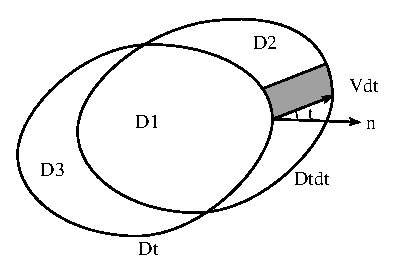
\includegraphics{../images/T1_Ch01-0002}
    \end{center}
    \caption{Illustration de la dérivée particulaire}  
    \label{fig:T1_Ch01-0002}
\end{figure}
\begin{figure}[ht]
    \begin{center}
        \subfloat[]{%
            \psfrag{dS}{$\mathrm{d}S$}
            \psfrag{e}{$\varepsilon$}
            \psfrag{n}{$\vec n$}
            \psfrag{n}{$\vec n$}
            \psfrag{-n}{$-\vec n$}
            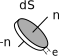
\includegraphics{../images/T1_Ch01-0003}
            \label{fig:T1_Ch01-0003}}
        \subfloat[]{%
            \psfrag{x1}{$x_1$}
            \psfrag{x2}{$x_2$}
            \psfrag{x3}{$x_3$}
            \psfrag{-e1}{$-\vec e_1$}
            \psfrag{-e2}{$-\vec e_2$}
            \psfrag{-e3}{$-\vec e_3$}
            \psfrag{M0}{\scriptsize $0$}
            \psfrag{M1}{\scriptsize $1$}
            \psfrag{M2}{\scriptsize $2$}
            \psfrag{M3}{\scriptsize $3$}
            \psfrag{n}{$\vec n$}
            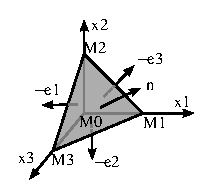
\includegraphics{../images/T1_Ch01-0004}
            \label{fig:T1_Ch01-0004}}
    \end{center}
    \caption{Flux}
\end{figure}
\end{document}
